\documentclass{article}
\usepackage{fancyhdr}
\usepackage{graphicx}
\usepackage{hyperref}
\usepackage{booktabs}
\usepackage{array}
\usepackage{amsmath}
\usepackage[table]{xcolor}
\usepackage{xcolor}
\usepackage{longtable}
\usepackage[a4paper, margin=1in]{geometry}
\usepackage{caption}
\usepackage{ulem}















\pagestyle{fancy}
\fancyhead[L]{Rapport de Soutenance : \textit{An Era of the Seas}}
\fancyfoot[L]{Dream Chasers}
\fancyfoot[C]{
    \begin{minipage}{1.5cm}
        \centering
        
\includegraphics[width=1cm]{logo.png}
    \end{minipage}
}
\fancyfoot[R]{\thepage}

\renewcommand{\footrulewidth}{0.1pt}
\renewcommand{\sectionmark}[1]{}
\renewcommand{\subsectionmark}[1]{}
\renewcommand{\contentsname}{}

\definecolor{lightblue}{HTML}{55FFFF}
\definecolor{pastelblue}{HTML}{097CA5}















\title{\textbf{Rapport de Soutenance}\\
\textbf{\textit{An Era of the Seas}}}
\author{%
    \begin{minipage}[c]{\textwidth}
        \centering
        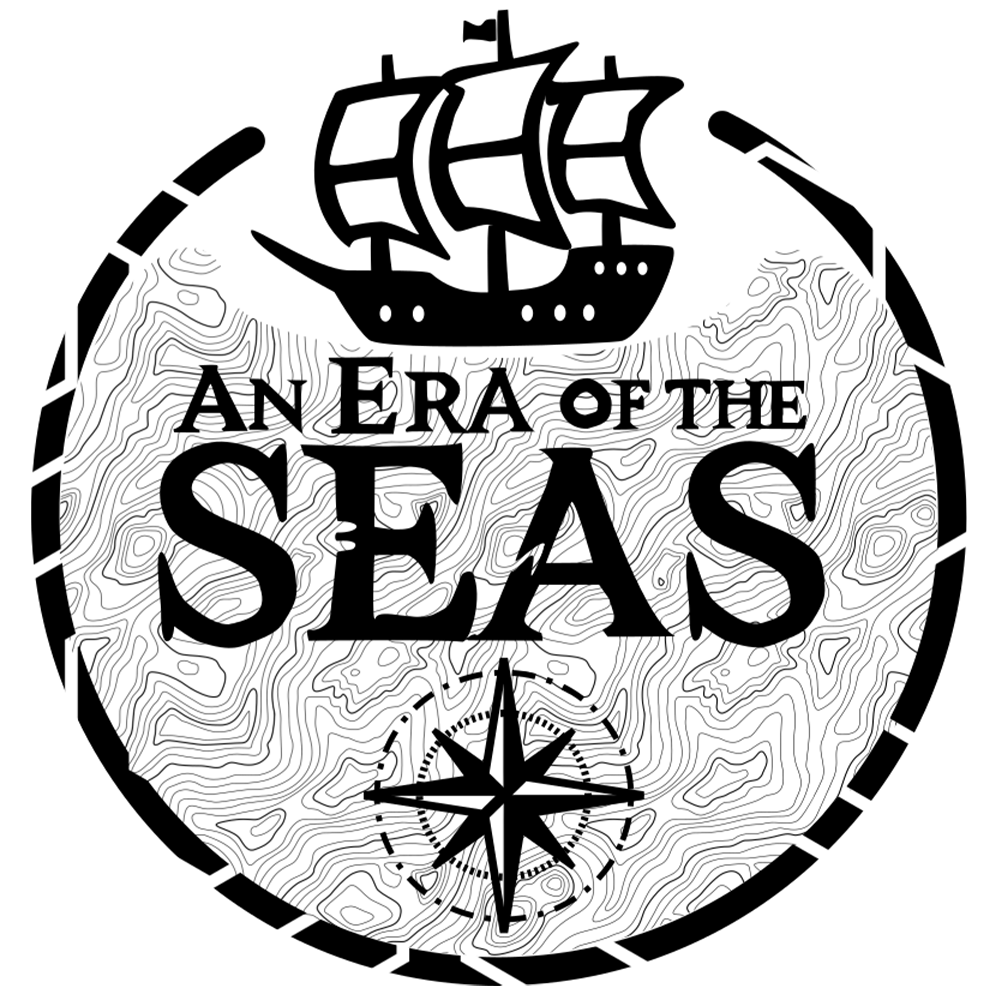
\includegraphics[width=3.5in]{AEotS Logo.png} \\
        \vspace{2cm}
        
\includegraphics[width=4in]{logo text.png}
    \end{minipage}
}
\date{}















\begin{document}

\maketitle

\vfill
\begin{center}
    \textbf{Lin Jérôme}\\
    \textbf{Ben Abdallah Achref}\\
    \textbf{Bruno Ethan}\\
    \textbf{Devin Joseph}\\
    \textbf{Classe : A1}
\end{center}













\newpage
\thispagestyle{empty}
\addtocounter{page}{-1}
\null















\newpage
\section*{Introduction}\hfill

Le projet \textit{An Era of the Seas} se distingue par son ambition de créer un monde maritime captivant, où l'aventure et l'exploration sont au cœur de l'expérience du jeu. Développé par l’équipe passionnée de \textbf{Dream Chasers}, ce roman visuel propose aux joueurs de se plonger dans l’univers fascinant de la navigation à voile, à travers des quêtes épiques et des défis stratégiques.\\

\textit{An Era of the Seas} place les joueurs dans la peau d’un capitaine qui doit parcourir des îles inexplorées, affronter des ennemis redoutables et reconstituer un héritage familial. Tout en naviguant sur les Shattered Seas, les joueurs découvriront un environnement vivant et évolutif, conçu pour offrir à chaque exploration un nouveau souffle. Le système de navigation réaliste, les améliorations du navire et la gestion de l’équipage sont autant d’éléments qui enrichissent l'expérience tout en plongeant le joueur dans un monde authentique et intrigant.\\

À travers ce projet, \textbf{Dream Chasers} souhaite offrir une expérience de jeu complète et immersive, alliant innovation technologique et profondeur narrative. L'équipe s'efforce de repousser les limites du développement de jeux vidéo pour proposer une aventure unique, riche en découvertes et en stratégies, qui captivera les amateurs de jeux d'exploration et de piraterie.

\newpage
\subsection*{Sommaire}
\tableofcontents















\newpage
\section{Origine et nature du projet}
\subsection{Origine}\hfill

Le projet du jeu \textit{An Era of the Seas} est le fruit d’un intérêt partagé entre les membres de l’équipe pour les jeux vidéo et le développement de logiciels. Cela implique une combinaison de connaissances en informatique et en développement de jeux vidéo pour créer une expérience captivante. Ce projet est une opportunité pour mettre en pratique les connaissances acquises dans la création d’un produit concret.

Développer un jeu est une opportunité d'acquérir des compétences dans différents domaines, de la programmation à la conception graphique, sans oublier la production sonore. Chaque membre peut contribuer avec ses compétences uniques, ce qui enrichit l'expérience collective.

L’essor de l’industrie du jeu vidéo et la croissance de son importance dans différents domaines tels que l’éducation et le divertissement ont également influencé la décision de créer un jeu. C’est l’occasion de s’immerger dans le secteur dynamique et en constante évolution du jeu vidéo.





\subsection{Informations du jeu} 
\subsubsection{Début et histoire du personnage principal}\hfill

\textit{An Era of the Seas} est un jeu dans lequel l’environnement maritime est primordial. Les joueurs incarneront le fils d’un grand et puissant marchand qui avait beaucoup d’influence et de contrôle sur les mers. Un jour, il reçoit une lettre lui informant que son père a péri durant une expédition mystérieuse. Il décide alors de découvrir ce qui lui est arrivé en débutant son aventure en tant que capitaine, il souhaite également restaurer la gloire de son père. Il découvrira la diversité des îles et commencera son voyage pour, non seulement, devenir un grand héros comme son père l’était, mais aussi trouver ses propres réponses.



\subsubsection{Objectifs du joueur}\hfill

Les joueurs pourront naviguer et découvrir les îles de Shattered Seas. Pour commencer cette aventure, le capitaine n'a qu’une barque en bois qu’il a trouvé sur la plage. Il devra aussi explorer les 8 différentes îles. Les joueurs commenceront sur la première île, où ils découvriront les caractéristiques principales, les fonctionnalités et l’histoire du fils du grand marchand. Ils y découvriront le chemin pour accomplir l’objectif final du capitaine. Le capitaine devra voyager et atteindre chaque île pour retrouver les trésors dispersés de son père pour prendre le contrôle de Shattered Seas. Après avoir exploré les 7 premières îles, le capitaine pourra enfin terminer son aventure sur la dernière île où les difficultés et les défis restent à venir.



\subsubsection{Fonctionnalités du jeu}\hfill

Ce jeu présente des fonctionnalités uniques liées à son environnement.

\paragraph{Quête principale}\hfill

Ce jeu est basé sur une histoire. Le joueur vivra l'histoire du capitaine et sera immergé dans l'univers maritime de ce jeu. Grâce à la quête principale, le joueur pourra ensuite suivre l'histoire du capitaine.

\paragraph{Quêtes secondaires}\hfill

La quête principale est l'histoire principale du capitaine, mais il existe aussi des histoires secondaires qui se déroulent au cours de son aventure à travers les mers et les îles. Ces quêtes peuvent aider le joueur à comprendre certaines fonctionnalités et offrent de généreuses récompenses. Ces quêtes consistent à accomplir des tâches, des livraisons, des combats contre certains ennemis spécifiques ou d'aider des résidents de Shattered Seas.

\paragraph{Système de navigation immersif}\hfill

Le bateau utilise le vent ou les rames pour naviguer en fonction du niveau du bateau et de l'équipage. Cela signifie naviguer avec des rames pour les bateaux ayant un niveau faible, puis suivre la direction du vent, régler les voiles et utiliser le gouvernail pour les bateaux ayant un niveau supérieur. Pour que le capitaine puisse se localiser et trouver un chemin vers un lieu spécifique, il utilisera une carte et une boussole.

\paragraph{Entretien et améliorations du bateau/navire}\hfill

Le bateau du joueur peut être amélioré en fonction de l’avancement dans la quête principale. Lorsque le bateau est endommagé, le joueur doit le réparer en utilisant des matériaux dans le but de pouvoir à nouveau naviguer sur les mers. Il peut acheter la base du bateau auprès d'un vendeur et l'améliorer avec certains matériaux.

\paragraph{Membres d’équipage}\hfill

Puisque le joueur incarne un capitaine naviguant sur les mers, il dispose de son propre équipage. Cet équipage est composé de différents membres aux tâches multiples qui ont été soigneusement recrutés dans les villes et des quêtes dans le but d'aider le capitaine dans son voyage. Chaque membre possède des statistiques spécifiques. Par conséquent, il est conseillé de les attribuer aux bonnes tâches au profit du parcours du capitaine. Par exemple, certains membres de l’équipage sont plus aptes à manier les rames, tandis que d’autres sont mieux adaptés à l’exploration.

\paragraph{Armes}\hfill

Pour pouvoir lutter contre les ennemis, le joueur a la possibilité d'utiliser des épées et des fusils. Les armes peuvent être obtenues dans des coffres au trésor, mais celles-ci sont courantes et peu puissantes. Il est recommandé d’en acheter chez un marchand dans les villes pour obtenir des armes avec de meilleures statistiques et infliger plus de dégâts.

\paragraph{Stigmata (Améliorations du joueur)}\hfill

Les Stigmata (Stigma au singulier) sont des marques inscrites sur la main avec l'aide d'un mage situé dans les villes. Ces marques améliorent les capacités du joueur (vitesse, attaque...). Elles peuvent être obtenues en les collectant dans des coffres au trésor ou en les achetant auprès du mage. Ces derniers ont investi beaucoup de temps et d’efforts dans la création des Stigmata. Par conséquent, les Stigmata vendus par les mages sont bien plus efficaces et plus puissants que ceux trouvés dans la nature. Par conséquent, acheter des Stigmata auprès d’un mage confère des statistiques nettement supérieures à celles obtenue dans les coffres au trésors. Cette qualité n'est évidemment pas sans impact sur le nombre de pièces du capitaine, celles-ci coûtent bien plus cher que ceux trouvés dans la nature.

\paragraph{Coffre au trésor}\hfill

Pour obtenir des ressources et des pièces, des coffres au trésor peuvent être découverts sur les îles et dans des zones gardées par des ennemis. Ces coffres contiennent des pièces de monnaie, des armes, des Stigmata ainsi que des objets pour améliorer le bateau, les armes et les Stigmata. Ces trésors aident le capitaine à établir une certaine richesse, et comme l'argent signifie le pouvoir dans Shattered Seas, cela lui permet d’accroître son influence sur les mers.

\paragraph{Villes}\hfill

Chaque île possède sa propre ville, où l’on trouve plusieurs types de commerçants : 
\begin{itemize}
    \item \textbf{Fabricants de bateaux et de navires :} Ils proposent leur superbes créations, des petits bateaux aux imposants navires. Selon l'île, ces concessionnaires proposent de meilleures coques et des meilleures améliorations de navires.
    \item \textbf{Fabricants d'armes :} Ils vendent des épées et des fusils performants pour affronter les ennemis.
    \item \textbf{Mages :} Ils peuvent utiliser leur magie mystique pour inscrire un Stigma que le capitaine possède ou qu’il a acheté. Ils vendent aussi leurs propres Stigmata, qui sont plus puissants.
    \item \textbf{Vendeurs de nourriture :} Ils vendent de la nourriture délicieuse aux habitants et aux aventuriers, afin de garantir qu'ils ne manquent pas d'énergie et ne meurent pas de faim.
\end{itemize}

\paragraph{Combat (PvE)}\hfill

Dans cette aventure, le chemin du capitaine n’est évidemment pas paisible, il rencontrera divers ennemis, tant sur les îles qu’à travers les mers. Pour se défendre et attaquer les ennemis, les armes, Stigmata et l’équipage seront utiles sur le terrain. Comme sur les mers, le bateau peut attaquer, et les membres d'équipage sont essentiels en la matière. Les statistiques des armes, des Stigmata, de l’équipage et du bateau sont donc essentielles pour infliger des dégâts et résister aux attaques des ennemis.

\paragraph{Multijoueur}\hfill

Ce jeu propose un mode multijoueur dans lequel le joueur pourra choisir une classe et jouer en fonction de celle-ci. Dans ce mode, aucun avantage lié à l'avancement ou aux objets du mode Solo n'est accordé au joueur.

\paragraph{Pêche}\hfill

Une mécanique amusante permettant au joueur d’obtenir des poissons utiles pour se nourrir et des trésors comme des pièces et des ressources. Cela sera possible grâce à une canne à pêche que le capitaine possède dès le début du jeu, et utilisable dans des plans d'eau assez vaste comme les lacs et les océans.





\subsection{Outils}
\subsubsection{Outils de gestion d’équipe}\hfill

Pour pouvoir communiquer efficacement sur différents aspects du développement du jeu entre les membres de l’équipe, il est crucial de disposer d’un outil dédié. Ainsi, un serveur Discord est particulièrement utile. Cela permet à l'équipe de communiquer facilement et d’organiser les discussions en différents canaux en fonction des sujets de développement spécifiques.\\

De plus, la gestion des tâches est essentielle pour maintenir le projet sur la bonne voie et suivre les progrès. Une liste de choses à faire peut s’avérer être très utile dans ce domaine. Elle peut fournir un aperçu clair des tâches à effectuer. Microsoft To Do est une excellente solution pour cela. Les tâches peuvent être attribuées à un membre de l'équipe et la date d'échéance peut être définie pour une tâche. Cela permet au membre de l'équipe d'être conscient de ce qui doit être fait, des délais et de maintenir sa productivité.



\subsubsection{Outils de développement du jeu}\hfill

Dream Chasers utilise GitHub pour pouvoir travailler efficacement ensemble en groupe sur le projet. Il permet à l’équipe de suivre les modifications apportées au code du jeu, garantissant ainsi que tout le monde travaille sur la dernière version sans écraser le travail des autres.\\

Le jeu est codé en C\# (Csharp) pour plusieurs raisons. C\# est un langage de programmation orienté objet, une caractéristique utile pour les jeux et C\# est également très souvent utilisé dans les moteurs de jeux comme Unity.\\

Pour l’IDE (Environnement de développement intègre), l’équipe utilise Rider de JetBrains car il présente divers avantages. Il est spécifiquement conçu pour le développement .NET (dotnet). Ici, l'équipe utilise dotnet core 7 pour développer le jeu. L'outil de débogage de Rider est très puissant, il facilite l'identification des problèmes dans le code grâce au débogage étape par étape et à la surveillance des variables. De plus, Rider fournit un éditeur Unity et est généralement plus rapide que certains autres IDE comme Visual Studio.\\

Le moteur de jeu utilisé est Unity, comme mentionné précédemment, pour de nombreuses raisons. Il offre une interface utilisateur accessible qui facilite la gestion des projets par les développeurs. Avec Unity, le jeu peut être pris en charge sur plusieurs plateformes. Ainsi, le jeu sera opérationnel même si le joueur utilise Windows, macOS ou Linux. Il fournit une variété d'outils et de fonctionnalités pour l'environnement 3D du jeu, y compris un moteur physique intégré.
















\newpage
\section{Objet d’étude}
\subsection{Intérêts et objectifs}\hfill

L'objectif principal du projet est de créer une expérience de jeu immersive, avec une histoire captivante et des mécanismes engageants. Grâce à ce projet, les membres de l'équipe pourront appliquer les connaissances et les concepts qu'ils ont appris dans un contexte réel et créatif. Le processus de création d'un jeu permet à l'équipe de surmonter des défis techniques et les encourage à développer des compétences pratiques en résolution de problèmes.





\subsection{Bénéfices communs}\hfill

Ce projet offre de nombreux avantages en équipe. 

Travailler avec les autres favorise une communication efficace entre les membres, une compétence cruciale dans le monde professionnel. Grâce à des discussions fréquentes, les membres de l’équipe développent la capacité à exprimer clairement leurs idées, à écouter les commentaires et à s’adapter à différentes perspectives.\\

De plus, le travail en équipe privilégie une meilleure coordination, avec une gestion des dépendances des tâches. Chaque membre de l'équipe peut se spécialiser dans certaines tâches, par exemple la programmation, la conception de jeux et l'ingénierie audio, ce qui améliore la productivité et l’efficacité. La division des tâches permet également au projet d’avancer plus rapidement, puisque les tâches peuvent être réalisées simultanément.\\

Enfin, le travail d’équipe conduit à des solutions plus innovantes et créatives. Le brainstorming peut générer une variété d’idées, se traduisant par des concepts et des mécanismes de jeu plus originaux et uniques.





\subsection{Bénéfices individuels}\hfill

Il existe aussi de nombreux avantages personnels à participer à ce genre de projet.

La création d’un jeu permet avant tout aux développeurs de maîtriser une technologie spécifique. Par exemple, les membres peuvent se concentrer sur différents aspects de la création d'un jeu, tels que la logique du jeu, le moteur physique, la conception et l'animation 3D, la conception sonore et bien d'autres.\\

De plus, les membres de l’équipe rencontreront inexorablement des défis techniques, des obstacles et des problèmes au cours du processus. La résolution de problèmes renforce les capacités de résolution de problèmes, qui est une compétence cruciale dans toute carrière en informatique. Surmonter ces défis renforce également la confiance et aide les membres à devenir plus adaptables.\\

Dans un projet collaboratif, chaque membre doit porter des responsabilités. Ils sont responsables de la qualité et de la ponctualité de leur travail. Cela peut renforcer le sentiment d’autonomie et d’appropriation. Ils doivent s’assurer que leurs contributions respectent les attentes et les délais de l’équipe. Cela aide à gagner en indépendance.\\

Participer à un projet de groupe nécessite une bonne gestion du temps. Cela signifie apprendre l’équilibre entre le travail personnel et les besoins du groupe. Les membres doivent planifier et prioriser leurs tâches, en veillant à contribuer à l’avancement du projet.\\

Enfin, travailler en groupe sur un projet de jeu permet aux membres d'acquérir des compétences techniques en communication. Les membres doivent expliquer clairement les idées, les solutions et le code complexes aux autres, en s'assurant que tout le monde comprenne bien. Cette capacité à communiquer des détails techniques de manière accessible est une compétence très utile,  qui sera très souvent sollicitée dans le monde professionnel.















\newpage
\section{Entreprise}
\subsection{Dream Chasers}\hfill

L’entreprise s'appelle \textbf{Dream Chasers}, un nom qui reflète l'esprit de l'entreprise, en quête de créer une expérience qui transforme les rêves les plus fous en réalité. L’entreprise pense que les jeux ne se limitent pas à un simple divertissement, ils constituent une porte d'entrée vers de nouveaux mondes, des aventures et la réalisation d'idées fantastiques. Le nom de l’entreprise est un hommage à ceux qui rêvent et à ceux qui souhaitent les poursuivre. 





\subsection{Spécificités}\hfill

Dream Chasers se distingue par leur capacité à fusionner compétences techniques et expression artistique. L’entreprise s’investi dans le développement des jeux qui engagent non seulement les joueurs sur le plan intellectuel, mais qui résonnent également sur le plan émotionnel. L’équipe est composée de développeurs, de concepteurs et de conteurs enthousiastes qui considèrent la création de jeux comme une forme d'art, alliant technologie de pointe, récits riches et environnements immersifs.

La méthodologie distinctive de Dream Chasers se caractérise par une attention méticuleuse aux détails, englobant tout, des mécanismes de jeu à la musique évocatrice qui améliore chaque scène. L’entreprise aspire à créer non seulement des jeux, mais aussi des expériences profondes qui laissent une impression durable sur les joueurs, les incitant à réfléchir à leur parcours longtemps après avoir terminé le jeu. 

De plus, Dream Chasers accorde la priorité à la collaboration et à l’innovation au sein de sa culture d’entreprise. Une atmosphère est cultivée pour permettre à la créativité de prospérer, offrant à chaque membre de l'équipe la possibilité d'influencer la trajectoire des projets. Cet esprit de collaboration favorise de nouvelles perspectives et une expérimentation continue, garantissant que chaque jeu développé est une aventure unique.





\subsection{Domaine d’activité}\hfill

Dream Chasers opère dans le domaine dynamique du développement de jeux vidéo, mais son champ d'action s'étend au-delà du jeu conventionnel. L’objectif principal réside dans la création de jeux d’aventure narratifs, tout en explorant les opportunités dans les technologies éducatives et les expériences de réalité virtuelle.

L’objectif de Dream Chasers est de créer des jeux qui éduquent et divertissent, en utilisant la narration interactive pour aborder des thèmes importants tels que la conscience environnementale, les récits historiques et la croissance personnelle. L’entreprise reconnaît le potentiel des jeux vidéo en tant qu’outils efficaces d’apprentissage et de développement, s’engageant à intégrer ces éléments dans ses projets à mesure qu’elle avance.





\subsection{A propos du jeu et de l’entreprise}\hfill

Avec ce jeu, Dream Chasers s’adresse aux joueurs en leur demandant s'ils se sont déjà interrogés sur ce que faisaient les pirates dans un passé lointain. Les joueurs peuvent ressentir de la nostalgie pour l'histoire de la navigation et des pillages dans les Caraïbes. C'est pourquoi l’équipe collabore étroitement avec la Nostalgic Pirates Association (NPA) pour développer ce jeu, qui vise à offrir une réminiscence rafraîchissante de l'atmosphère et de la piraterie des Caraïbes au XVIIIe siècle. Cela redonnera vie à tous les capitaines qui vivaient à cette époque. Les pirates nostalgiques sont invités à se demander s'il n'existe pas un mode de vie plus épanouissant que celui de partager un verre avec des équipiers amicaux sur le pont. Ensemble, ils pourront respirer l'air marin iodé, découvrir des îles enchanteresses et inexplorées, explorer les sept mers et se lancer à la recherche de magnifiques trésors.

Chez Dream Chasers, il existe un véritable engagement à répondre aux préoccupations des esprits des pirates nostalgiques, c'est pourquoi l’entreprise aide ceux qui ne peuvent plus poursuivre leurs rêves à les réaliser derrière un roman visuel grâce au jeu \textit{An Era of the Seas}, conçu pour les rêveurs des mers.















\newpage
\section{Equipe}\hfill

Pour ce jeu, il est crucial d’inclure des personnes aux talents et spécialités variées, afin d’offrir aux joueurs le monde dont ils rêvent.

\subsection{Jérôme}\hfill

Toujours proche des villes dès son plus jeune âge, il aspire à comprendre à quel point l'environnement naturel peut être paisible. Il choisit sa propre voie en explorant l'industrie du jeu vidéo et aspire à réaliser ses propres ambitions en créant avec d'autres des mondes imaginaires. Dans ce projet, il dirigera l'équipe pour réaliser la création d'un magnifique monde maritime. Il est également responsable de la mise en place des objets, des récompenses, des coffres, des armes, des bateaux, des statistiques des Stigmata et de la gestion des comptes.





\subsection{Achref}\hfill

Passionné par la culture geek depuis son enfance, son personnage s'est façonné en jouant à des jeux vidéo et en regardant plusieurs animés. En plus de cela, son expérience dans le vaste monde de la programmation l'a conduit dans le monde du développement de jeux, en mettant l'accent sur les jeux basés sur une histoire et les jeux de rôle.





\subsection{Ethan}\hfill

Depuis son enfance jusqu’à aujourd’hui, Ethan a toujours cherché à comprendre comment fonctionnait le monde qui l’entourait et comment quelqu’un pouvait interagir avec ce monde. La création d'un environnement avec sa propre physique et sa logique représente une parfaite opportunité pour développer sa compréhension. Il supervisera l'environnement du jeu, tel que la simulation de l'eau, la météo et la physique.





\subsection{Joseph}\hfill

Élevé dans la ville balnéaire du Havre, Joseph a appris à aimer l'océan et souhaite explorer ce thème avec ses coéquipiers au cours de ce projet. Comme il navigue depuis longtemps, il est principalement chargé de l'implémentation du système de navigation dans le jeu. Joseph est ainsi chargé de mettre en place le vent, la gestion des voiles, le système de localisation et tout ce qui touche à l'océan et à la navigation.















\newpage
\section{Distribution des tâches}
\begin{table}[h]
    \centering
    \begin{tabular}{|>{\columncolor{pastelblue!60}}l|c|c|c|c|}
        \hline
        \rowcolor{pastelblue!60}
        \textbf{Tâhes} & \textbf{Jérôme} & \textbf{Achref} & \textbf{Ethan} & \textbf{Joseph}\\
        \hline
        Menu \& UI & \cellcolor{blue}R &  & \cellcolor{cyan}S &\\
        \hline
        Simulation de l'eau & & & \cellcolor{blue}R & \cellcolor{cyan}S\\
        \hline
        Simulation de la météo & & \cellcolor{blue}R & \cellcolor{cyan}S &\\
        \hline
        Mouvements (bateau, joueur...) & & & \cellcolor{cyan}S & \cellcolor{blue}R\\
        \hline
        Mouvements IA (ennemis, mouvements, attaques) & & \cellcolor{blue}R & & \cellcolor{cyan}S\\
        \hline
        Carte & \cellcolor{cyan}S & & \cellcolor{blue}R &\\
        \hline
        Système de localisation (carte, bousole...) & & \cellcolor{cyan}S & & \cellcolor{blue}R\\
        \hline
        Statistiques des objets & \cellcolor{blue}R & & & \cellcolor{cyan}S\\
        \hline
        Système de pêche & \cellcolor{cyan}S & \cellcolor{blue}R & &\\
        \hline
        Système de faim & & \cellcolor{cyan}S & \cellcolor{blue}R &\\
        \hline
        Réseau & \cellcolor{blue}R & \cellcolor{cyan}S & &\\
        \hline
        Multijoueur & \cellcolor{cyan}S & & & \cellcolor{blue}R\\
        \hline
        Histoire(Lore) & & & \cellcolor{cyan}S & \cellcolor{blue}R\\
        \hline
        Quêtes & & \cellcolor{cyan}S & \cellcolor{blue}R &\\
        \hline
        Site Web & & \cellcolor{blue}R & & \cellcolor{cyan}S\\
        \hline
        Design des entités & & \cellcolor{blue}R & \cellcolor{cyan}S &\\
        \hline
        Animations des entités & \cellcolor{cyan}S & & \cellcolor{blue}R &\\
        \hline
        SFX & \cellcolor{blue}R & & & \cellcolor{cyan}S\\
        \hline
        Musiques & \cellcolor{blue}R & \cellcolor{cyan}S & &\\
        \hline
        Optimisation du code & \cellcolor{blue}R & \cellcolor{blue}S & \cellcolor{blue}S & \cellcolor{blue}S\\
        \hline
        Correction de la langue & \cellcolor{cyan}S & & & \cellcolor{blue}R\\
        \hline
        Tests & \cellcolor{blue}R & \cellcolor{blue}R & \cellcolor{blue}R & \cellcolor{blue}R\\
        \hline
    \end{tabular}
\end{table}

\begin{itemize}
    \item \textcolor{blue}{R : Responsable}
    \item \textcolor{cyan}{S : Supléant}
\end{itemize}















\newpage
\section{Avancement et planification}
\begin{longtable}{|>{\columncolor{pastelblue!60}}l|l|c|c|c|}
    \hline
    \rowcolor{pastelblue!60}
    \textbf{Date limite} & \textbf{Tâches} & \textbf{Progrès} & \textbf{Responsable} & \textbf{Supléant}\\
    \hline
    27/10/2024 & Statistiques des objets & 25\% & Jérôme & Joseph\\
    \hline
    \multicolumn{5}{|c|}{\cellcolor{pastelblue!60}\textbf{Examens B1 (28-31/10/2024)}}\\
    \hline
    03/11/2024 & Carte & 80\% & Ethan & Jérôme\\
    \hline
    10/11/2024 & Simulation de l'eau & 50\% & Ethan & Joseph\\
    \hline
    10/11/2024 & Statistiques des objets & 50\% & Jérôme & Joseph\\
    \hline
    10/11/2024 & Améliorations des objets & 25\% & Jérôme & Joseph\\
    \hline
    10/11/2024 & Site Web & 80\% & Achref & Joseph\\
    \hline
    17/11/2024 & Menu pricipal & 40\% & Jérôme & Ethan\\
    \hline
    24/11/2024 & Menu pricipal & 80\% & Jérôme & Ethan\\
    \hline
    24/11/2024 & Système de localisation & 80\% & Joseph & Achref\\
    \hline
    01/12/2024 & Mouvenments du joueur & 50\% & Joseph & Ethan\\
    \hline
    08/12/2024 & UI du joueur & 25\% & Jérôme & Ethan\\
    \hline
    15/12/2024 & Système de localisation & 100\% & Joseph & Achref\\
    \hline
    22/12/2024 & UI du joueur & 50\% & Jérôme & Ethan\\
    \hline
    22/12/2024 & Mouvenments du joueur & 80\% & Joseph & Ethan\\
    \hline
    22/12/2024 & SFX & 20\% & Jérôme & Joseph\\
    \hline
    29/12/2024 & Animations des entités & 10\% & Ethan & Jérôme\\
    \hline
    28/12/2024 & Deplacement des entités/IA & 20\% & Achref & Joseph\\
    \hline
    29/12/2025 & Carte & 100\% & Ethan & Jérôme\\
    \hline
    29/12/2024 & Mouvements du bateau & 50\% & Joseph & Ethan\\
    \hline
    05/01/2025 & Design des entités & 25\% & Achref & Ethan\\
    \hline
    05/01/2025 & Mouvements du bateau & 80\% & Joseph & Ethan\\
    \hline
    05/01/2025 & Simulation de la météo & 50\% & Achref & Ethan\\
    \hline
    05/01/2025 & Simulation de l'eau & 80\% & Ethan & Joseph\\
    \hline
    \multicolumn{5}{|c|}{\cellcolor{pastelblue!60}\textbf{Examens B2 (6-10/01/2025)}}\\
    \hline
    12/01/2025 & Histoire & 40\% & Joseph & Ethan\\
    \hline
    12/01/2025 & Quête principal & 40\% & Ethan & Achref\\
    \hline
    \multicolumn{5}{|c|}{\cellcolor{pastelblue!60}\textbf{Première Soutenance technique (13-17/01/2025)}} \\
    \hline
    12/01/2025 & Site Web & 100\% & Achref & Joseph\\
    \hline
    19/01/2025 & UI du joueur & 100\% & Jérôme & Ethan\\
    \hline
    26/01/2025 & Statistiques des objets & 100\% & Jérôme & Joseph\\
    \hline
    02/02/2025 & SFX & 40\% & Jérôme & Joseph\\
    \hline
    02/02/2025 & Déplacements des entités/IA & 50\% & Achref & Joseph\\
    \hline
    02/02/2025 & Design des entités & 50\% & Achref & Ethan\\
    \hline
    02/02/2025 & Quête principale & 75\% & Ethan & Achref\\
    \hline
    09/02/2025 & Simulation de la météo & 100\% & Achref & Ethan\\
    \hline
    16/02/2025 & Animations des entités & 50\% & Ethan & Jérôme\\
    \hline
    02/03/2025 & Déplacements des entités/IA & 80\% & Achref & Joseph\\
    \hline
    02/03/2025 & Design des entités & 80\% & Achref & Ethan\\
    \hline
    02/03/2025 & SFX & 60\% & Jérôme & Joseph\\
    \hline
    \multicolumn{5}{|c|}{\cellcolor{pastelblue!60}\textbf{Examens B3 (03-07/03/2025)}}\\
    \hline
    10/03/2025 & Quête principale & 100\% & Ethan & Achref\\
    \hline
    10/03/2025 & Histoire & 80\%\ & Joseph & Ethan\\
    \hline
    \multicolumn{5}{|c|}{\cellcolor{pastelblue!60}\textbf{Deuxième Soutenance technique (10-14/03/2025)}} \\
    \hline
    30/03/2025 & Système de pêche & 100\% & Achref & Jérôme\\
    \hline
    30/03/2025 & Système de faim & 100\% & Ethan & Achref\\
    \hline
    20/04/2025 & Déplacements des entités/IA & 100\% & Achref & Joseph\\
    \hline
    04/05/2025 & Animations des entités & 100\% & Ethan & Jérôme\\
    \hline
    25/05/2025 & Histoire & 100\% & Joseph & Ethan\\
    \hline
    \multicolumn{5}{|c|}{\cellcolor{pastelblue!60}\textbf{dernière Soutenance technique (26-30/05/2025)}}\\
    \hline
\end{longtable}















\newpage
\section{Cahier des charges technique}
\begin{itemize}
    \item Nom du groupe : Dream Chasers
    \item Nom du projet : \textit{An Era of the Seas}
\end{itemize}





\begin{longtable}{|l|l|l|c|}
    \caption*{\textbf{\uline{Noms des membres}}}\\
    \hline
    \rowcolor{pastelblue!60}
    Nom & Prénoms & Login & Classe\\
    \hline
    Ben Abdallah & Achref & achref.ben-abdallah & A1\\
    \hline
    Bruno & Ethan & ethan.bruno & A1\\
    \hline
    Devin & Joseph & joseph.devin & A1\\
    \hline
    Lin & Jérôme & jerome.lin & A1\\
    \hline
\end{longtable}





\begin{longtable}{|c|c|c|c|c|}
    \caption*{\textbf{\uline{Type de jeu}}}\\
    \hline
    \cellcolor{lightblue}Action/Aventure & Battle Royale & Beat them all & Combat & Simulation\\
    \hline
    \cellcolor{lightblue}FPS & MMORPG & MOBA & Party Games & Survival Horror\\
    \hline
    Plateforme & Puzzles & Reflexion & Rogue Like & TPS\\
    \hline
    \cellcolor{lightblue}RPG & RTS & Sandbox & Shoot them up & Course\\
    \hline
    Autre : & \multicolumn{4}{|c|}{}\\
    \hline
\end{longtable}





\begin{longtable}{|>{\columncolor{pastelblue!60}}l|l|l|l|l|}
    \caption*{\textbf{\uline{Caractéristiques}}}\\
    \hline
    \multicolumn{5}{|c|}{\cellcolor{pastelblue!60}\textbf{Caractéristiques générales du jeu}}\\
    \hline
    IA & \cellcolor{lightblue}Errer & \cellcolor{lightblue}Attaquer & \cellcolor{lightblue}S'échapper & "Path Finder"\\
    \hline
    Multijoueur & \cellcolor{lightblue}Coopératif & Battle (2-4) & \multicolumn{2}{|l|}{Massif}\\
    \hline
    Réseau & P2P & Lan & \multicolumn{2}{|l|}{\cellcolor{lightblue}Online}\\
    \hline
    \multicolumn{5}{|c|}{\cellcolor{pastelblue!60}\textbf{Caractéristiques graphiques}}\\
    \hline
    Dimension & 2D & \cellcolor{lightblue}3D & Autres : &\\
    \hline
    Particularités & Stéreoscopie & AR & \multicolumn{2}{|l|}{VR}\\
    \hline
    Graphiques & \cellcolor{lightblue}Perso & Custom & \multicolumn{2}{|l|}{\cellcolor{lightblue}Existant}\\
    \hline
    Précisions : & \multicolumn{4}{|c|}{}\\
    \hline
    \multicolumn{5}{|c|}{\cellcolor{pastelblue!60}\textbf{Caractéristiques sonores}}\\
    \hline
    Musique & Perso & Custom & \multicolumn{2}{|l|}{\cellcolor{lightblue}Existant}\\
    \hline
    FX & Perso & \cellcolor{lightblue}Custom & \multicolumn{2}{|l|}{Existant}\\
    \hline
    Précisions : & \multicolumn{4}{|c|}{Thème musicale orienté vers l'univers maritime}\\
    \hline
    \multicolumn{5}{|c|}{\cellcolor{pastelblue!60}\textbf{Autres caractéristiques}}\\
    \hline
    Site Web & Perso & \cellcolor{lightblue}Custom & \multicolumn{2}{|l|}{Préfabriqué}\\
    \hline
\end{longtable}







\begin{figure}[h]
    \caption*{\textbf{\uline{Diagramme de GANTT}}}
    \centering
    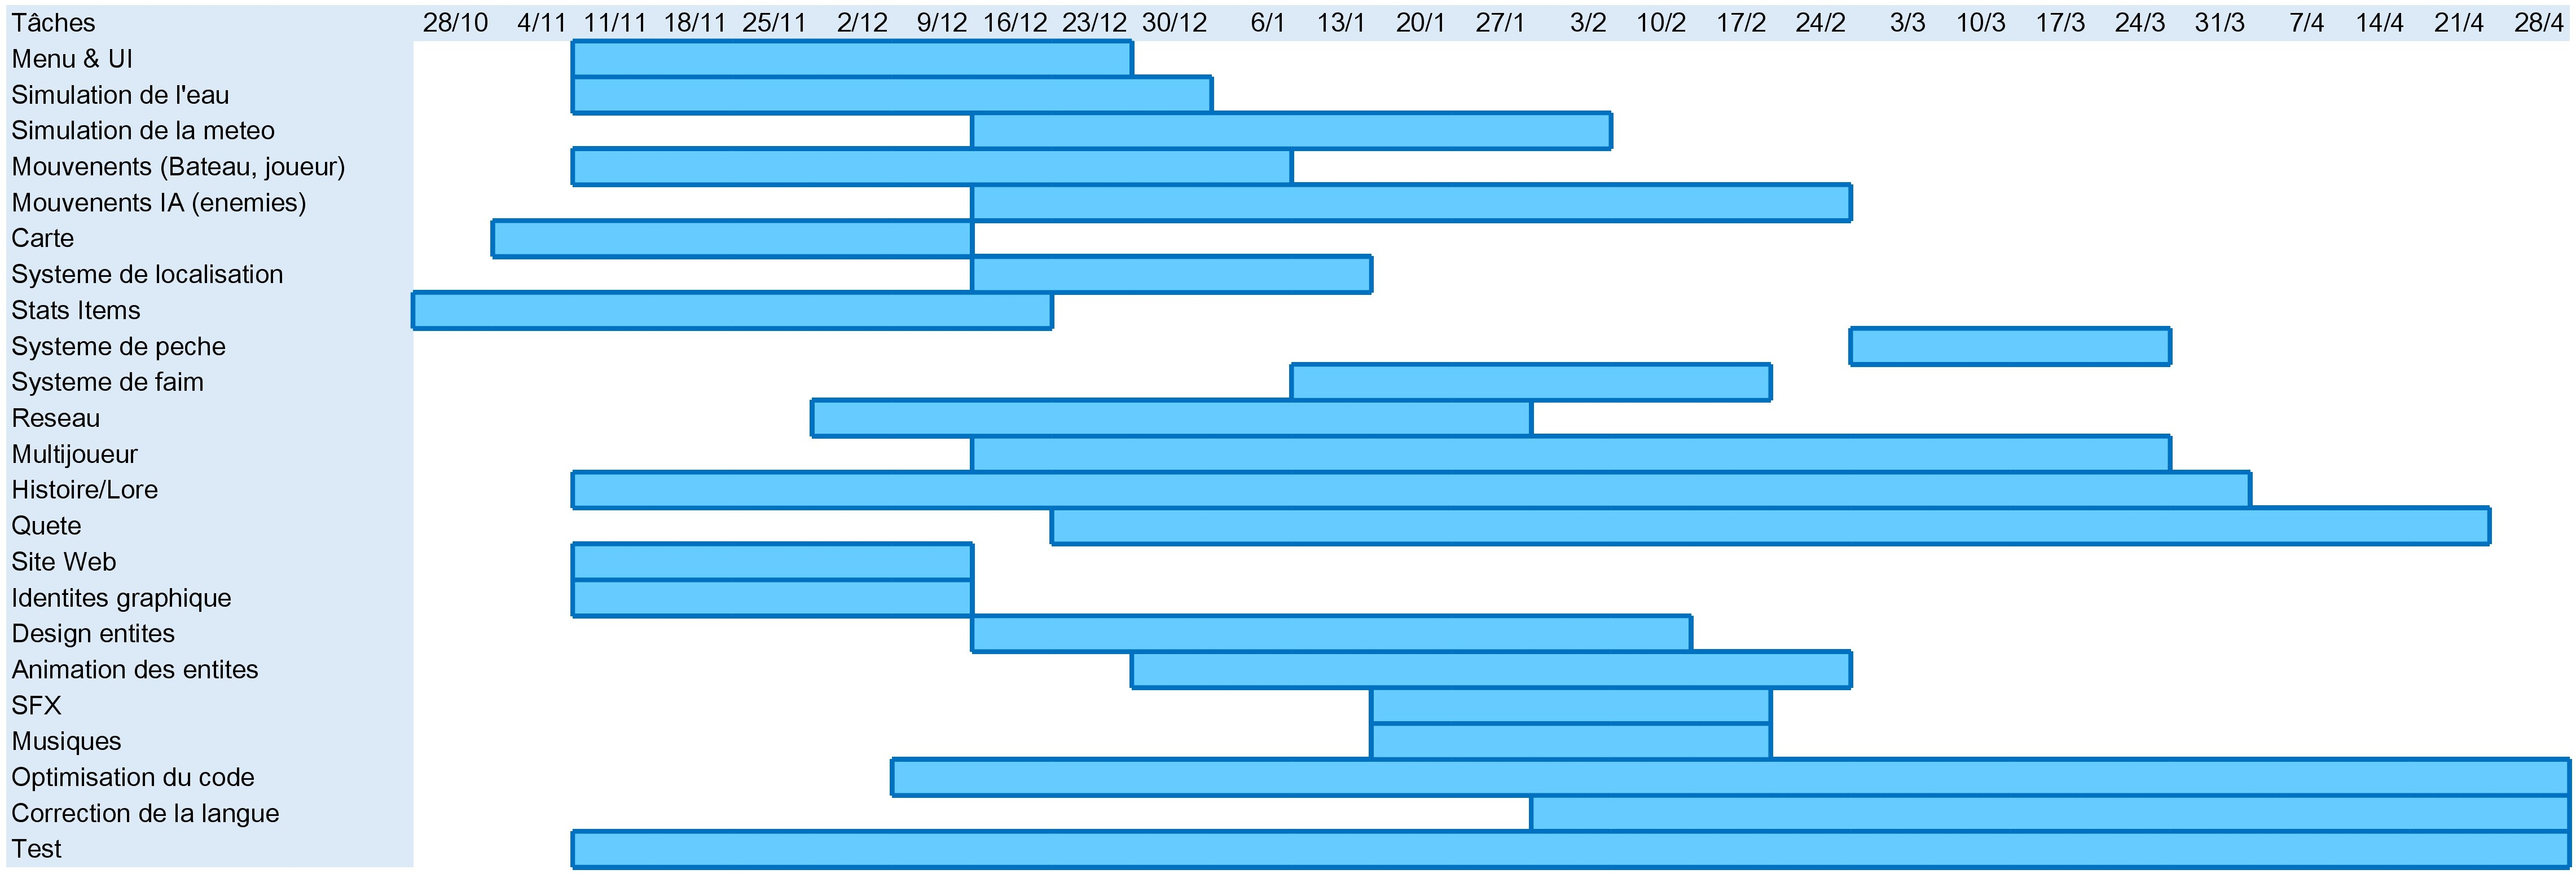
\includegraphics[angle=90, width=3.22in]{gant.png}
    \label{fig:mon_image}
\end{figure}















\clearpage
\section{Récit de la réalisation}\hfill
\subsection{Jérôme}\hfill
\subsubsection{Implémentation des objets dans le jeu}\hfill

Le développement du jeu a commencé par une étape cruciale : lister tous les objets du jeu. Ces objets étaient variés : des armes comme des épées et des armes à feu, des stigmata, des bateaux, des membres d’équipage, ainsi que divers matériaux comme des pièces, des gouttes d’eau pure, du bois et de l’acier. Le plus difficile dans cette phase initiale a été de trouver des noms originaux et captivants pour ces objets. Cela m’a demandé un véritable effort d’inspiration, avec de longues recherches sur Internet pour enrichir ma créativité.\\

Une fois cette étape franchie, j’ai entrepris de structurer ces informations dans un fichier JSON. Heureusement, je maîtrisais déjà la manipulation de fichiers JSON, ce qui a rendu cette étape relativement simple et rapide.\\

Ensuite, j’ai dû passer à une tâche plus complexe : concevoir un document Excel pour définir les statistiques de base du joueur en fonction des niveaux, en sachant que le niveau maximum est de 100. Il fallait aussi déterminer les matériaux nécessaires pour améliorer le niveau du joueur. Trouver les formules adéquates s’est avéré être un véritable casse-tête. J’ai exploré des modèles de croissance exponentielle et linéaire, en définissant des statistiques précises pour le niveau 1 et le niveau 100. Malgré mon aisance sur Excel, cette phase a nécessité une recherche approfondie sur Internet, car les formules que je recherchais étaient très spécifiques.\\

Après avoir finalisé les statistiques du joueur, je suis passé à la définition des statistiques pour chaque type d’objet. Armé des formules déjà établies, cette partie s’est révélée plus rapide, bien que répétitive. Néanmoins, j’ai dû, à plusieurs reprises, ajuster les statistiques des niveaux 1 et 100 pour maintenir un équilibre cohérent avec les statistiques du joueur.\\

Une fois toutes les données prêtes, il était temps de les exporter des fichiers Excel (.xlsx) vers des fichiers CSV (.csv). Cette conversion était essentielle pour pouvoir manipuler les données en C\# et les charger dans Unity par la suite.\\

Puis est venue une étape décisive : écrire les scripts pour intégrer les objets du jeu dans Unity. Cela impliquait de manipuler les fichiers JSON et CSV. J’ai découvert et utilisé deux bibliothèques très populaires pour cette tâche : Newtonsoft.Json pour les fichiers JSON et CsvHelper pour les fichiers CSV.\\

Pour bien comprendre comment charger les données, j’ai exploré la documentation de ces bibliothèques et regardé plusieurs vidéos explicatives sur YouTube. Le traitement des fichiers JSON m’a donné du fil à retordre, tandis que celui des fichiers CSV s’est avéré plus intuitif.\\

Une fois les fonctions de chargement prêtes, il me fallait les exécuter dans Unity via des scripts MonoBehaviour. Cette étape a ouvert la porte à de nombreux défis. L’un des problèmes majeurs était de définir une méthode efficace pour communiquer les données entre les scripts. Une fois cette méthode trouvée, un autre obstacle est apparu : les scripts ne se chargeaient pas dans le bon ordre. Pour résoudre ce problème, j’ai dû modifier les paramètres d’exécution des scripts dans le profil du jeu Unity.\\

Une fois les problèmes de chargement des scripts réglés et l’ensemble fonctionnant correctement, il était temps de m’attaquer à une autre étape essentielle : la gestion des données du joueur.\\

Au départ, j’avais envisagé d’utiliser Firebase Realtime Database pour sauvegarder les informations du joueur. Cependant, j’ai rapidement réalisé qu’il était impossible d’intégrer les bibliothèques nécessaires, disponibles sur NuGet, dans un projet Unity. Face à cet obstacle, j’ai décidé de me tourner vers une solution locale : sauvegarder les données du joueur sous forme de fichiers JSON. Cette approche m’avait déjà été suggérée lors de mes recherches sur la gestion des sauvegardes dans Unity.\\

Le fichier JSON devait contenir plusieurs éléments cruciaux : la position du joueur, son niveau et son inventaire. Concernant l’inventaire, j’avais déjà réfléchi à une organisation logique : faire la distinction entre les objets équipés par le joueur et ceux simplement stockés dans son inventaire.\\

Avec cette structure en tête, j’ai commencé à écrire un script permettant de gérer ces données. Il devait charger les informations depuis le fichier JSON et les traduire en un objet C\# exploitable. Une fois les données chargées, il fallait recalculer les statistiques du joueur, en prenant en compte les différents bonus apportés par les stigmata et l’arme qu’il avait équipée.\\

Cette partie s’est avérée plus intuitive que je ne l’imaginais. La majorité des recherches nécessaires avait déjà été effectuée lors des étapes précédentes, et j’avais également écrit les scripts pour charger les données des objets. Il ne me restait plus qu’à exploiter ces données pour ajuster les statistiques du joueur.\\

Ce processus, bien que technique, s’est déroulé de manière fluide. Il était gratifiant de voir le système fonctionner comme prévu et d’observer les statistiques du joueur évoluer dynamiquement en fonction des objets qu’il équipait.\\

Cette étape a marqué une avancée significative dans le développement de mon jeu, me rapprochant encore un peu plus de ma vision finale. Chaque défi surmonté, chaque ligne de code écrite, renforce ma compréhension et mon enthousiasme pour ce projet.\\



\subsubsection{Menu \& Interface utilisateur}\hfill

Avant de plonger dans Unity, j’ai pris le temps de me documenter. J’ai consulté des guides et regardé plusieurs vidéos sur YouTube pour comprendre comment créer des menus et des interfaces utilisateur dans Unity. À première vue, cela semblait relativement simple, mais je savais qu’il faudrait porter une attention particulière à la manière de présenter les boutons et les éléments de l’UI. Mon objectif était de créer une interface claire et intuitive qui n’entraverait pas l’expérience du joueur.\\

\paragraph{Conception du Menu Principal}\hfill

J’ai commencé par placer les boutons et le fond du menu principal. Trouver un background adapté s’est avéré assez rapide grâce à l’Asset Store de Unity. J’y ai découvert un ensemble d’images qui correspondaient parfaitement au thème maritime de mon jeu.\\

En revanche, trouver des boutons prêts à l’emploi qui me convenaient a été plus compliqué. Ne trouvant rien à mon goût, j’ai décidé de les concevoir moi-même. Ayant une expérience en photomontage, j’ai créé des boutons personnalisés et sélectionné une police en harmonie avec l’esthétique générale du jeu.\\

L’intégration de ces boutons dans Unity a été une étape formatrice. Au départ, je ne comprenais pas comment remplacer les sprites par défaut des boutons Unity. Je tentais simplement de glisser et déposer mes fichiers d’images sur l’espace réservé aux sprites, mais cela ne fonctionnait pas. Après quelques recherches, j’ai découvert qu’il fallait convertir les fichiers d’images en sprites avant de pouvoir les utiliser. Une fois cette étape maîtrisée, j’ai pu appliquer mes créations et donner au menu principal un aspect visuel unique et immersif.\\

\paragraph{Scripts pour la Navigation dans l’UI}\hfill

La prochaine étape consistait à écrire des scripts pour gérer les interactions entre les différents éléments du menu. Je devais permettre à l’utilisateur de changer de canvas ou d’afficher et cacher des GameObjects selon ses actions. Cette partie a été relativement simple grâce à une fonction intégrée dans Unity, et les recherches nécessaires pour comprendre son fonctionnement ont été rapides.\\

\paragraph{Conception du Menu Inventaire}\hfill

Le vrai défi de l’interface utilisateur s’est présenté lors de la création du menu inventaire. Ce menu devait afficher dynamiquement les objets que le joueur possédait, un système bien plus complexe que le menu principal. Heureusement, j’ai trouvé une vidéo qui expliquait exactement ce que je voulais réaliser. En suivant ce tutoriel, j’ai pu comprendre les étapes nécessaires et surmonter les difficultés sans trop de problèmes.\\



\subsubsection{Organisation}\hfill

Dès le début du projet, j’ai pris l’initiative de me porter volontaire comme chef de projet, motivé par mon sens de l’organisation et ma rigueur. Cette responsabilité m’a permis de structurer les étapes du développement et de guider mon équipe vers l’objectif final.\\

\paragraph{Définition des Tâches et Élaboration d’un Planning}\hfill

La première étape consistait à définir les différentes tâches à accomplir, ce qui s’est avéré relativement simple. Une fois les tâches identifiées, il a fallu les répartir entre les membres de l’équipe et s’accorder sur leur répartition.\\

Le véritable défi a été de créer un planning clair et visuel. Au départ, je me suis contenté d’un tableau conforme aux exigences du cahier des charges, avec les pourcentages des tâches associées. Cependant, cette représentation manquait de lisibilité et n’était pas optimale pour le suivi du projet. J’ai donc opté pour un diagramme de Gantt, beaucoup plus visuel et compréhensible. Grâce à Excel, la création de ce diagramme a été à la fois rapide et efficace, facilitant la communication avec les autres membres de l’équipe.\\

\paragraph{Ajustements Après le Premier Cahier des Charges}\hfill

Après la remise du premier cahier des charges technique, j’ai constaté quelques déséquilibres dans la répartition des tâches. Certains membres exerçaient plus de responsabilités que d’autres. J’ai donc révisé la répartition en apportant des ajustements mineurs et en consultant les autres membres pour valider ces modifications.\\

\paragraph{Problèmes d’Assiduité}\hfill

Un autre défi organisationnel est survenu lorsqu’un des membres de l’équipe n’a pas respecté les délais pour ses tâches. Une semaine avant la soutenance méthodologique, la carte 2D et le logo du jeu n’étaient toujours pas terminés. Face à cette situation, j’ai dû prendre en charge la création de la carte 2D moi-même, tandis que le logo, réalisé par ce membre, est arrivé tardivement.\\

\paragraph{Départ d’un Membre Avant la Soutenance}\hfill

Le problème le plus conséquent s’est produit la veille de la soutenance méthodologique : l’un des membres, Matteo Bollot, a annoncé qu’il quittait l’établissement. Ce départ soudain nous a confrontés à un nouvel obstacle : assurer un temps de parole équitable entre les membres restants lors de la soutenance. Grâce à la réactivité des autres membres, nous avons rapidement trouvé une solution pour réorganiser l’oral, et celui-ci s’est déroulé sans encombre.\\

À la suite du départ de Matteo, l’équipe a été réduite à quatre membres. Après la soutenance, j’ai dû réarranger la répartition des tâches pour répartir équitablement la charge de travail supplémentaire. J’ai pris soin de consulter les autres membres avant de finaliser ces ajustements. Bien que chaque membre ait désormais un peu plus de travail, j’ai décidé de conserver la planification initiale en espérant que chacun respecterait ses engagements.\\

Cette expérience en tant que chef de projet m’a confronté à des défis humains et organisationnels variés, mais elle m’a également permis de renforcer mes compétences en gestion de groupe. Malgré les imprévus, l’équipe reste soudée, et nous continuons à progresser vers la finalisation de notre jeu vidéo.\\





\subsection{Achref}





\subsection{Ethan}





\subsection{Joseph}



















\newpage
\section{Conclusion}\hfill

Pour conclure le projet \textit{An Era of the Seas}, développé par Dream Chasers, nous avons exploré les nombreux aspects qui définissent la création de ce jeu. Ce projet repose sur une passion commune pour la création de jeux immersifs et l'exploration de thématiques maritimes captivantes. L'équipe multidisciplinaire de Dream Chasers, composée de développeurs, designers et artistes talentueux, s'efforce de créer une expérience unique en combinant un scénario engageant, des mécaniques de jeu innovantes et une forte collaboration.\\

Ce projet offre non seulement l'opportunité d'acquérir des compétences pratiques dans divers domaines (programmation, conception graphique, production sonore), mais il reflète également l'esprit d'innovation de Dream Chasers. Chaque membre de l'équipe est encouragé à apporter ses compétences spécifiques, permettant ainsi de relever les nombreux défis techniques du développement tout en stimulant la créativité.\\

Ainsi, \textit{An Era of the Seas} incarne à la fois un défi technique et une aventure humaine, dans laquelle l'équipe Dream Chasers aspire à offrir aux joueurs une expérience mémorable. C'est une démonstration de la capacité des Dream Chasers à transformer des idées ambitieuses en une réalité interactive, marquant non seulement les joueurs, mais aussi les membres de l'équipe qui auront grandi au cours de cette aventure.







\end{document}